\section{C++}

\begin{figure}[H]
	\centering 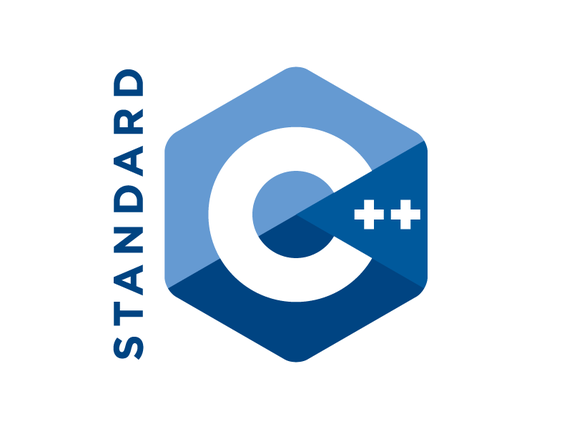
\includegraphics[scale=0.3]{images/c++.png}
	\caption{C++ Logo}
\end{figure}

C++ is a general-purpose programming language. It has imperative, object-oriented and generic programming features, while also providing facilities for low-level memory manipulation.

It was designed with a bias toward system programming and embedded, resource-constrained and large systems, with performance, efficiency and flexibility of use as its design highlights. C++ has also been found useful in many other contexts, with key strengths being software infrastructure and resource-constrained applications, including desktop applications, servers (e.g. e-commerce, web search or SQL servers), and performance-critical applications (e.g. telephone switches or space probes). C++ is a compiled language, with implementations of it available on many platforms and provided by various organizations, including the Free Software Foundation (FSF's GCC), LLVM, Microsoft, Intel and IBM.

C++ is standardized by the International Organization for Standardization (ISO), with the latest standard version ratified and published by ISO in December 2014 as ISO/IEC 14882:2014 (informally known as C++14). The C++ programming language was initially standardized in 1998 as ISO/IEC 14882:1998, which was then amended by the C++03, ISO/IEC 14882:2003, standard. The current C++14 standard supersedes these and C++11, with new features and an enlarged standard library. Before the initial standardization in 1998, C++ was developed by Bjarne Stroustrup at Bell Labs since 1979, as an extension of the C language as he wanted an efficient and flexible language similar to C, which also provided high-level features for program organization.

In 1979, Bjarne Stroustrup, a Danish computer scientist, began work on "C with Classes", the predecessor to C++. The motivation for creating a new language originated from Stroustrup's experience in programming for his Ph.D. thesis. Stroustrup found that Simula had features that were very helpful for large software development, but the language was too slow for practical use, while BCPL was fast but too low-level to be suitable for large software development. When Stroustrup started working in AT\&T Bell Labs, he had the problem of analyzing the UNIX kernel with respect to distributed computing. Remembering his Ph.D. experience, Stroustrup set out to enhance the C language with Simula-like features. C was chosen because it was general-purpose, fast, portable and widely used. As well as C and Simula's influences, other languages also influenced C++, including ALGOL 68, Ada, CLU and ML.

Initially, Stroustrup's "C with Classes" added features to the C compiler, Cpre, including classes, derived classes, strong typing, inlining and default arguments.[10]

In 1983, "C with Classes" was renamed to "C++" (++ being the increment operator in C), adding new features that included virtual functions, function name and operator overloading, references, constants, type-safe free-store memory allocation (new/delete), improved type checking, and BCPL style single-line comments with two forward slashes (//). Furthermore, it included the development of a standalone compiler for C++, Cfront.

In 1985, the first edition of The C++ Programming Language was released, which became the definitive reference for the language, as there was not yet an official standard. The first commercial implementation of C++ was released in October of the same year.

In 1989, C++ 2.0 was released, followed by the updated second edition of The C++ Programming Language in 1991. New features in 2.0 included multiple inheritance, abstract classes, static member functions, const member functions, and protected members. In 1990, The Annotated C++ Reference Manual was published. This work became the basis for the future standard. Later feature additions included templates, exceptions, namespaces, new casts, and a boolean type.

After the 2.0 update, C++ evolved relatively slowly until, in 2011, the C++11 standard was released, adding numerous new features, enlarging the standard library further, and providing more facilities to C++ programmers. After a minor C++14 update released in December 2014, various new additions are planned for July 2017 and 2020.

Many other programming languages have been influenced by C++, including C\#, D, Java, and newer versions of C (after 1998).

Features of Language:
\begin{enumerate}
	\item \textbf{Object storage}: As in C, C++ supports four types of memory management: static storage duration objects, thread storage duration objects, automatic storage duration objects, and dynamic storage duration objects.
	\begin{enumerate}
		\item \textbf{Static storage duration objects}: Static storage duration objects are created before main() is entered (see exceptions below) and destroyed in reverse order of creation after main() exits. The exact order of creation is not specified by the standard (though there are some rules defined below) to allow implementations some freedom in how to organize their implementation. More formally, objects of this type have a lifespan that "shall last for the duration of the program".
		\item \textbf{Thread storage duration objects}: Variables of this type are very similar to static storage duration objects. The main difference is the creation time is just prior to thread creation and destruction is done after the thread has been joined.
		\item \textbf{Automatic storage duration objects}: The most common variable types in C++ are local variables inside a function or block, and temporary variables. The common feature about automatic variables is that they have a lifetime that is limited to the scope of the variable. They are created and potentially initialized at the point of declaration (see below for details) and destroyed in the reverse order of creation when the scope is left.
		\item \textbf{Dynamic storage duration objects}: These objects have a dynamic lifespan and are created with a call to new and destroyed explicitly with a call to delete.
	\end{enumerate}
	\item \textbf{Templates}: C++ templates enable generic programming. C++ supports function, class, alias and variable templates. Templates may be parameterized by types, compile-time constants, and other templates. Templates are implemented by instantiation at compile-time. To instantiate a template, compilers substitute specific arguments for a template's parameters to generate a concrete function or class instance. Some substitutions are not possible; these are eliminated by an overload resolution policy described by the phrase "Substitution failure is not an error" (SFINAE). Templates are a powerful tool that can be used for generic programming, template metaprogramming, and code optimization, but this power implies a cost. Template use may increase code size, because each template instantiation produces a copy of the template code: one for each set of template arguments, however, this is the same or smaller amount of code that would be generated if the code was written by hand.[43] This is in contrast to run-time generics seen in other languages (e.g., Java) where at compile-time the type is erased and a single template body is preserved.\\
	\item \textbf{Objects}: C++ introduces object-oriented programming (OOP) features to C. It offers classes, which provide the four features commonly present in OOP (and some non-OOP) languages: abstraction, encapsulation, inheritance, and polymorphism. One distinguishing feature of C++ classes compared to classes in other programming languages is support for deterministic destructors, which in turn provide support for the Resource Acquisition is Initialization (RAII) concept.
	\begin{enumerate}
		\item \textbf{Encapsulation}: Encapsulation is the hiding of information to ensure that data structures and operators are used as intended and to make the usage model more obvious to the developer. C++ provides the ability to define classes and functions as its primary encapsulation mechanisms. Within a class, members can be declared as either public, protected, or private to explicitly enforce encapsulation. A public member of the class is accessible to any function. A private member is accessible only to functions that are members of that class and to functions and classes explicitly granted access permission by the class ("friends"). A protected member is accessible to members of classes that inherit from the class in addition to the class itself and any friends.\\
		\item \textbf{Inheritance}: Inheritance allows one data type to acquire properties of other data types. Inheritance from a base class may be declared as public, protected, or private. This access specifier determines whether unrelated and derived classes can access the inherited public and protected members of the base class. Only public inheritance corresponds to what is usually meant by "inheritance". The other two forms are much less frequently used. If the access specifier is omitted, a "class" inherits privately, while a "struct" inherits publicly. Base classes may be declared as virtual; this is called virtual inheritance. Virtual inheritance ensures that only one instance of a base class exists in the inheritance graph, avoiding some of the ambiguity problems of multiple inheritance.
	\end{enumerate}
	\item \textbf{Operators and operator overloading}: C++ provides more than 35 operators, covering basic arithmetic, bit manipulation, indirection, comparisons, logical operations and others. Almost all operators can be overloaded for user-defined types, with a few notable exceptions such as member access (. and .*) as well as the conditional operator. The rich set of overloadable operators is central to making user-defined types in C++ seem like built-in types.\\
	\item \textbf{Polymorphism}: Polymorphism enables one common interface for many implementations, and for objects to act differently under different circumstances.\\
	C++ supports several kinds of static (resolved at compile-time) and dynamic (resolved at run-time) polymorphisms, supported by the language features described above. Compile-time polymorphism does not allow for certain run-time decisions, while runtime polymorphism typically incurs a performance penalty.
	\begin{enumerate}
		\item Static polymorphism
		\item Dynamic polymorphism
		\begin{enumerate}
			\item Inheritance
			\item Virtual member functions
		\end{enumerate}
	\end{enumerate}
\item Lambda expressions
\item \textbf{Exception handling}: Exception handling is used to communicate the existence of a runtime problem or error from where it was detected to where the issue can be handled. It permits this to be done in a uniform manner and separately from the main code, while detecting all errors. Should an error occur, an exception is thrown (raised), which is then caught by the nearest suitable exception handler. The exception causes the current scope to be exited, and also each outer scope (propagation) until a suitable handler is found, calling in turn the destructors of any objects in these exited scopes. At the same time, an exception is presented as an object carrying the data about the detected problem.\\
The exception-causing code is placed inside a try block. The exceptions are handled in separate catch blocks (the handlers); each try block can have multiple exception handlers, as it is visible in the example below.
\end{enumerate}
